\chapter{Introduction}\label{chap:introduction}
\begin{chapabstract}

Intro intro intro intro.

\end{chapabstract}

\section{Star Formation Rate (SFR)}

Star formation in galaxies is one of the most complex processes.
In modern astronomy, understanding it and its evolution is still a challenging problem.
To explain these, we need an advanced knowledge of dark matter and baryon physics.
The evolution of dark matter is now interpreted by the ``$\Lambda$ CDM (Cold Dark Matter) model'' which indicates structures in the universe have been forming hierarchically (bottom-up) \citep{Peebles1982}.
This model explains that a galaxy forms in a small dark halo once and merge into other halos to form larger systems as time goes on \citep{Blumenthal1984}.
With the advance of computational methods, a cosmological simulation can model this scenario and reproduce structures in the universe \citep[e.g.,][]{Navarro2000, Vale2004}.
However, the baryon evolution inside dark halos is much more difficult to understand because its evolution attributes to the composition of different scale of physics.
Revealing these physics needs as a first step to find constraints by measuring the star formation activity accurately.
When we measure the star formation activity at each era in the universe, we can constrain the galaxy evolution scenario observationally.
The star formation rate (SFR) is the total mass of stars formed in a galaxy per year, and it is typically used for representing the star formation activity in a galaxy.
SFR is one of the most fundamental and important values for understanding the galaxy evolution.

Here, we present the SFR calibration methods.
The fundamental equation to calculate SFR at time $t$ from intrinsic stellar luminosity at wavelength of $\lambda$ is shown below \citep{Buat1991}:

\begin{equation}\label{eq:Buat1991eq1}
    L\brp{\lambda,\,t}=\int_{0}^{t} \int_{\mr{M}\msb{low}}^{\mr{M}\msb{up}} F_{\lambda}\brp{m, \theta}\,\mr{SFR}\brp{t-\theta}\,\psi\brp{m}\,\mr{d}m \mr{d} \theta
\end{equation}
where $F_{\lambda}\brp{m, \theta}$ is the evolutionary stellar tracks, $\psi\brp{m}$ is the Initial Mass Function (IMF;~\citealt{Salpeter1955, Kroupa2001, Chabrier2003}), $\mr{SFR}\brp{t-\theta}$ is SFR at time $t-\theta$.
$\mr{M}\msb{up}$ $\brp{\mr{M}\msb{low}}$ is the upper (lower) limit of the stellar mass considered for the calculation.

Indeed, we can calculate SFR from Equation~\ref{eq:Buat1991eq1} in two ways.
One way is to assume a certain stellar synthesis model and star formation history, and to calculate parameters to reproduce luminosities which we can observe at present.
This method is called SED fitting and it is useful even for the galaxies experienced not stable star formation recently.
However, this method highly depends on the star formation history chosen for the calculation.

Another way is simple and to assume that $\mr{SFR}$ is constant over a certain timescale $T$ and SFR is proportional to the luminosity.
The timescale $T$ depends on the wavelength for measuring SFR\@.
In this case, we can measure SFR with the following equation:

\begin{equation}\label{eq:Buat1991sfrproportion}
    \mr{SFR} = C \times L\brp{\lambda}
\end{equation}
where $C$ is constant.

This method is simple and easy to measure SFR from a certain luminosity, but the assumption of the constant SFR is sometimes problematic.
Previous research show the required time to reach the steady state and SFR is $\sim\mr{Myr}$ for recombination lines ($\mr{H\alpha}, \mr{H\beta}$), $\sim 100\,\mr{Myr}$ for the ultraviolet emission and $\sim 1000\,\mr{Myr}$ for optical-near IR emissions \citep{Kennicutt1998, Kennicutt2012}.
These result show that the SFR calculated from Equation~\ref{eq:Buat1991sfrproportion} is different from the true value if SFR in a galaxy varies among $\sim 100\,\mr{Myr}$.
Although this simple calibration has the uncertainty of the assumption and also strongly depends on the IMF, standard calibrations for Equation~\ref{eq:Buat1991sfrproportion} are calculated with a spectral synthesis code and widely used for measuring SFR\@.

% write about dust attenuation

In this study, I investigate the calibration using the low-frequency radio emission around $\sim 100\MHz$.





\section{Cosmic Star Formation History}

Dr.\ Beatrice M. Tinsley proposed the galaxy evolution in her PhD thesis, titled ``Evolution of galaxies and its significance for cosmology''.

With 

\begin{figure}[htbp]
	\centering
	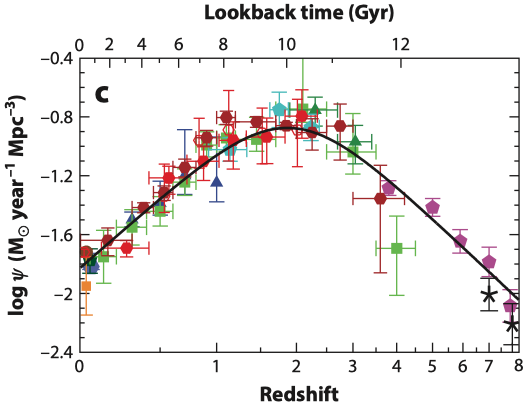
\includegraphics[width=.6\linewidth]{Chapter_1/Figures/Madau2014_Figure9.png}
    \caption[Reprint from Madau \& Dickinson 2014 (Figure~9)]{\label{fig:Madau2014_figure9}
        (Reprint from Madau \& Dickinson 2014, Figure~9)\\
    }
\end{figure}





\section{Low radio frequencies and SFR}
%\section{Background}
%
%The low-frequency radio emission from star-forming galaxies has been studied for many years.
%In this paper, we use the term ``Low frequency'' as the frequency less than a few GHz.
%The importance of this emission increased after the global log-linear correlation with infrared (IR) had been found.
%This correlation was discovered by \citet{Helou1985} using integrated far-infrared (FIR;\@$60\,\micron$ and $100\,\micron$) and $1.4\GHz$ radio luminosities in star-forming galaxies, and called the IR-Radio Correlation (IRC).
%\citet{Condon1991a,Yun2001a, Bell2003} have examined this global correlation using a different sample set and found it holds the tightness across more than three orders of magnitude.
%Recently, the low-frequency survey at around $100\MHz$ was operated by the LOw Frequency Array (LOFAR;~\citealt{VanHaarlem2013}) and the Murchison Widefield Array (MWA;~\citealt{Tingay2013a}).
%With the advent of these telescopes, \citet{CalistroRivera2017a, Read2018, Wang2019} extend the IRC study to at an order of magnitude lower frequency and find IRC is held at not only $1.4\GHz$ but $\sim 100\MHz$.
%
%Thanks to this correlation, we can regard the low frequency emission as a SFR indicator because IR luminosity is emitted by heated dust grains in a galaxy and can measure the SFR\@.
%Since the low-frequency emission is not affected by the dust extinction \citep{Yun2001a, Murphy2011} and it will be observed from a distant galaxies by the future extended survey, we anticipate its usefulness and need a further investigation of the relation between the radio and IR luminosities, especially its frequency dependence.
%However, the spatially-resolved studies show that a star-forming galaxy emits the radio emission whose spectral index depends on the galaxy region \citep{Kapinska2017a, For2018a, Heesen2019}.
%This means that the radio emission is sensitive to the local density environment of the ISM and it is not guaranteed a simple frequency dependence of the global relation between the integrated radio and IR luminosities.
%
%The integrated radio emission in star-forming galaxies across $100\MHz$ to $1.4\GHz$ is supposed to compose of a few percent to $10\%$ free-free and the synchrotron radiations \citep{Condon1992a}.
%Each radiation is emitted by electrons interacted with the electric field of ions in the \ih~region or the magnetic field in a galaxy.
%For emitting the synchrotron radiation, an electron needs to be accelerated to the light speed by the supernova remnant.
%While the synchrotron emission is expected to be dominant at these low frequencies, previous studies find the sign of the free-free absorption and flatter or turnover spectral \citep{Schober2017, Chyzy2018}.
%If the radio emission has a significant turnover among low frequencies, IRC does not have a simple frequency dependence and the radio emission is no longer useful as a SFR indicator.
%
%In this study, we investigate nearby star-forming galaxies from the reference sample for ensuring the reliability of measuring the SFR from the low-frequency emission.
%For examining the general trend, we use star-forming galaxy samples from Herschel Reference Survey (HRS;~\citealt{Boselli2010}) catalog which are supposed to represent the galaxy samples and the low-frequency emission from The GaLactic Extragalactic All-sky MWA (GLEAM;~\citealt{Hurley-Walker2017a}) Survey which observes the mJy scale radio emission from large areas with their 20 narrow bands.

This paper is organized as follows.
In Chapter~\ref{chap:data}, we introduce our galaxy samples and the low-frequency emissions used in this study.
In Chapter~\ref{chap:mmthod}, we introduce the IR-Radio Correlation with the $\qn$ value defined for evaluating the correlation quantitatively. Here, we also mention the way to investigate its frequency dependence and derive the radio SFR\@.
In Chapter~\ref{chap:results}, we show our results about the frequency dependence of IRC and the consistency of the radio SFR\@.
In Chapter~\ref{chap:discussions}, we compare our results with previous studies.
Finally, we summarize our study in Chapter~\ref{chap:summary}.



%\bibliographystyle{mnras}
%%\bibliography{example} % if your bibtex file is called example.bib
%\bibliography{masterthesis}




%Reference Table \ref{tab:Table1}.  And blah blah blah.
%
%\begin{table}[t]
%\caption[TOC Table Description]{Caption.}
%	\centering
%	\begin{tabular}{lcc}
%		\hline
%        {\textbf{Setting}}                      & \multicolumn{2}{c}{\textbf{Mt C/y}} \\
%		                                                           &         Min          &     Max      \\ \hline
%		AAA                         &          40          &      66      \\
%		BBB                               &          14          &      66      \\
%		CCC                                       &          18          &      43      \\
%		DDD      &          4           &    $>$12     \\
%		EEE                                  &          0           &      47      \\
%		FFF                    & 1$ \times $10$^{-4}$ &      52      \\
%		GGG &          8           &      42      \\ \hline
%	\end{tabular}
%    \label{tab:Table1}
%\end{table}
%
%\section{Figures}
%Reference Figure~\ref{fig:Fig1}.
%
%\subsection{This is a subsection}
%\begin{figure}[t]
%	\centering
%	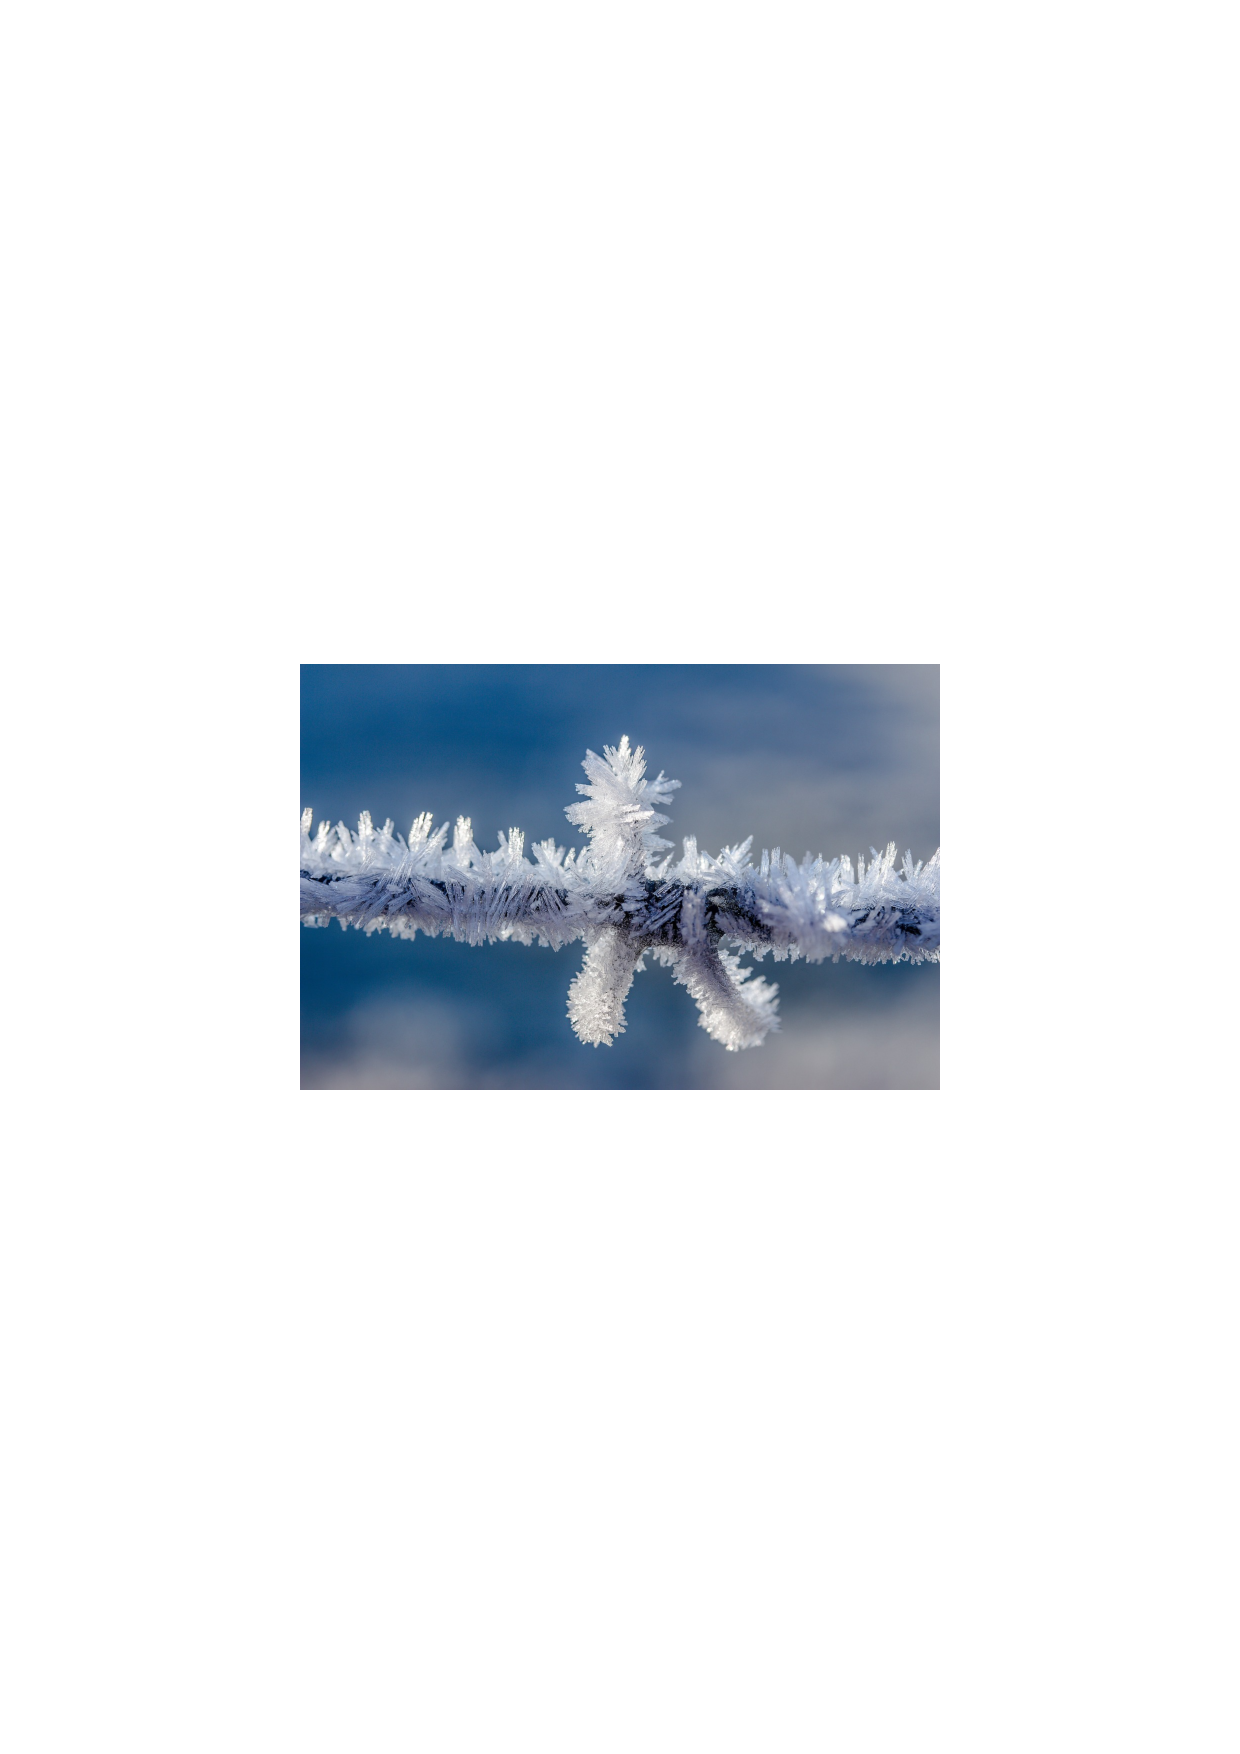
\includegraphics[width=.6\linewidth]{sFigs/Fig1.pdf}
%	\caption[TOC Figure Description]{Caption.}
%	\label{fig:Fig1}
%\end{figure}
%\subsubsection{This is a subsubsection}
%Citations are like \cite{goossens93,AbedonHymanThomas2003}.  Or maybe \cite{Abedon1994} said something.  Or \cite{Cerveny} which is an example of how to make a bib file that includes an author whose name begins with a non-English character and \cite{forgues96}: an example of referencing a Ph.D. thesis and yet more non-English characters.




%\bibliographystyle{abbrvnat}
%\bibliography{Chapter_1/ref1}
